\chapter{基于规则匹配与大语言模型的工具图谱构建}

\section{引言}

本章介绍了一种结合规则匹配与大语言模型的工具图谱构建方法,并基于该方法成功实现了一个大规模的工具图谱。围绕工具图谱构建中的关键挑战,本章重点解决以下几个问题:首先,针对数据清洗问题,探讨了如何从调用路径数据中筛选出高质量的工具集合和有效的工具调用路径,以保证图谱构建的基础数据可靠性;其次,设计了工具图谱的本体模型,用以清晰表达工具之间的依赖关系;然后,提出了一种结合规则匹配与大语言模型的方法,自动从工具描述文档和调用数据中提取工具图谱实例模型的关键信息;接着,介绍了如何将整理后的数据导入到Neo4j数据库中,实现高效的图谱存储与查询;最后,针对工具图谱的动态性和可扩展性,讨论了图谱更新机制,尤其是在新增工具节点或修改工具关系时如何高效地更新图谱实例。

\section{可行性分析}

在实际的工具调用场景中,不同类型的工具之间通常存在一定的顺序关系和依赖关系。这些依赖关系隐含在工具调用路径中的“过程性知识”中,对工具规划具有重要的启发作用。这些知识不仅揭示了工具之间的调用关系和跳转逻辑,还可以为大语言模型在工具调用时提供关键的决策辅助。因此,本文希望通过对工具之间的转换关系进行建模,缩小工具搜索范围至更精确的空间,从而提升工具调用的效率和准确性。

为了验证这一假设,我们分析了目前公开可用的通用工具学习数据集ToolBench\cite{Qin2023} 和 API-Bank\cite{Li2023c},这些数据集中包含了大量的多跳工具调用路径。我们随机抽取了一组API工具,通过人工分析其文档及代码测试,发现工具之间确实存在不同程度的参数依赖关系。例如,“淘宝商品ID搜索”和“淘宝商品评论”的API工具之间共享一个“淘宝商品ID”的参数。在获取商品评论之前,必须先调用“淘宝商品ID搜索”获取商品ID,否则无法进行后续操作。我们将这种依赖定义为“强参数依赖”,即后续工具调用完全依赖于前一个工具的输出。

除此之外,还有一些工具之间存在较弱的参数依赖关系,例如“城市经纬度查询”和“根据经纬度获取实时天气”的工具。虽然它们之间共享经纬度参数,但这些参数也可以通过其他途径获得。因此,我们将这类依赖定义为“弱参数依赖”。此外,还存在一种时序依赖关系,这种关系可能与参数依赖共存,体现为工具调用路径中隐含的顺序约束。例如,某些工具在特定任务链中必须按照既定顺序调用才能完成任务。

通过对工具调用路径的整体分析,我们进一步验证了这一猜想:每个工具的后续调用中仅有少数后继工具被频繁使用。这表明工具调用路径中确实蕴含了丰富的工具关系数据,可以供我们构建工具知识图谱使用。

\section{整体流程}

基于这一发现,本文从开源工具调用路径数据中进行筛选与清洗,通过制定两种策略——基于工具的筛选与基于调用路径的筛选,筛选出高质量的工具调用路径数据,作为知识图谱构建的数据来源。

在此基础上,我们设计了知识图谱的本体模型结构,对工具之间的依赖关系进行建模,定义了三种核心依赖关系,用于表达工具之间的依赖关系。
随后,我们结合规则匹配和大语言模型的提示词设计,开发了一套自动化知识抽取流程,从工具描述文档和调用路径数据中构建工具知识图谱。
通过上述流程获得的实例数据被导入到 Neo4j 数据库中。Neo4j的高效图数据存储和可视化功能,不仅能够直观展示图谱的结构,也为后续工具图谱的查询奠定了基础。
最后,由于工具场景是复杂多变的,我们需要对工具图谱进行动态的更新,针对该问题本文提出了图谱更新方法,提供了高效的更新策略来保证图谱的实时性和有效性。

\section{数据收集和清洗}

\subsection{数据集介绍}

在大语言模型工具调用研究中,存在许多公开的数据集,这些工具数据集通常包括工具的描述文档(例如JSON格式\cite{Qin2023}或OpenAPI规范(OAS)\cite{Song2023}格式)、工具调用路径\cite{Qin2023, liu2024toolace}以及路径的正确性标签等丰富信息。这些数据集为大语言模型工具调用的性能评估和模型优化提供了重要的基准数据。

\sloppy
目前常见的工具调用数据集包括ToolBench\cite{Qin2023}、API-Bank\cite{Li2023c}、
TaskBench\cite{shen2023taskbench}和ToolAce\cite{liu2024toolace}等。
这些数据集在工具数量、工具文档格式、调用复杂度以及场景覆盖方面具有各自的特点。
\relax

在本研究中,选择ToolBench作为主要数据集,主要因为其工具覆盖范围广、采用真实API工具、易于访问和调用路径数据丰富等优势。ToolBench包含49个类别、共计16464个RESTful API工具,覆盖范围广泛,工具描述详细。
此外,ToolBench的数据来源于真实世界的API工具,这些工具不仅能够直接调用,其中部分甚至是免费的,有利于降低成本和使用门槛。同时,基于真实环境的API工具和响应数据使本研究更具工程与实践意义。
同时,ToolBench中的API通过统一的密钥(key)即可调用,无需额外的注册或复杂的鉴权步骤,大大降低了工具使用的门槛,便于集成到本文的系统中。
更重要的是,ToolBench提供了丰富的工具调用路径数据,共计126486条路径。这些路径数据都经过了工具评价器器ToolEval\cite{Qin2023}的标记,能够从中筛选得到成功执行的路径。

ToolBench的整体构造基于开放的API托管平台“RapidAPI Hub”,其API工具以层级化结构组织。从大类别(如天气、金融、翻译等)到工具集(tool collections),再到具体的API工具,层层递进。用户通过订阅工具集即可访问对应的API工具。数据集还包含多种类型的信息,例如工具集的详细描述(名称、描述、类别等)、工具输入输出参数列表、示例代码和工具调用路径数据。这些信息为研究工具调用任务提供了全面支持。在本研究中,重点使用了ToolBench中的工具调用路径数据,构建了工具图谱。这些路径数据记录了工具协作完成任务的调用顺序和逻辑关系,为工具图谱的构建奠定了坚实的基础。

值得说明的是,RapidAPI Hub上的API工具往往具有一定的功能相似性,多个工具可以在功能上互为替代。因此,对于同一用户任务,通常存在多条调用路径可以达到目标结果。这种路径的多样性使得任务解决方案并非唯一,而是具备灵活性和鲁棒性。研究中通过分析调用路径的输出结果是否符合预期,评估路径的合理性,即判断一组API调用是否能够满足任务需求。这种多路径、多结果的特性为研究工具调用的动态性和灵活性提供了更多维度的分析依据,进一步推动了多工具协作的深入探索。

\subsection{数据清洗}

\subsubsection{工具节点筛选}

% 在筛选高质量API工具之前,我们首先限定了工具的应用领域,聚焦于购物、旅游、天气和餐饮四个类别。这些类别的API工具功能丰富,为用户提供了广泛的应用场景支持。

由于在后续的工具选择阶段,大语言模型会针对工具的描述文档来进行选择,工具描述的信息丰富程度和清晰程度将会是
影响工具选择准确性的重要因素之一。因此我们在进行图谱构建前,应该先对API文档的描述信息丰富度进行评估和筛选。

由于原始数据中的API工具数量较大,完全依赖人工评估不仅耗时较长,而且不同评估者之间的理解差异会导致评分标准难以统一。为了解决这些问题,我们引入了大语言模型,对工具的描述信息进行自动化评分,同时设计了一套量化的评分标准,以评估信息丰富度。这种方法不仅节省了时间和成本,还通过细粒度的打分规则和提示词,确保了评分标准的一致性,从而提高了分数的参考价值。

在分析中发现,低质量的API描述文档通常存在内容不完整和语义不清晰两个问题。因此,我们围绕这两个维度对API描述进行评价和筛选:完整性(如是否详细说明功能)和易读性(如是否语义清晰)。这种系统化的评估方式,有助于更高效地筛选出高质量的API描述文档。

每个维度的分数范围为1到3分,其中:
\begin{itemize}
    \item 1分:不满足要求;
    \item 2分:基本满足要求,但有一定的不清晰或者不完整;
    \item 3分:描述非常详细,语言清晰流畅,信息完整且丰富。
\end{itemize}

由于初始数据中的工具集较大,我们可以严格地筛选在两个维度得分都为3的工具,仅留下语义清晰的、功能完整的工具。

为验证大语言模型的打分可靠性,我们抽样了100个API的信息提交给3位人工评审员进行独立打分,并与大语言模型的打分结果进行了对比分析。

一致性(Consistency)在此处定义为人工打分与大语言模型打分结果的完全一致性。如果人工评审员与大语言模型对同一API的打分在某一维度上相同,则认为该API在该维度的评分是一致的。表中的一致性百分比是根据以下公式计算的:

\[
\text{一致性 (\%)} = \frac{\text{人工与大模型打分相同的API数量}}{\text{总API数量}} \times 100
\]

该指标用于量化大语言模型评分与人工评审之间的匹配程度,从而验证模型评分的可靠性。

表\ref{tab:api_score_comparison}展示了两者在不同维度下的评分分布及一致性。

\begin{table}[h]
  \centering
  \bicaption{人工标记与模型标记分数一致性}{Comparison of Human and Model Scoring Distribution}
  \label{tab:api_score_comparison}
  \begin{tabular}{l|c|c|c}
  \toprule
  \textbf{Dimension} & \textbf{Score} & \textbf{Human Count} & \textbf{Model Count} \\ \midrule
  \multirow{3}{*}{Completeness} & 1 & 20 & 22 \\ 
                                & 2 & 40 & 38 \\ 
                                & 3 & 40 & 40 \\ \hline
  \textbf{Completeness Consistency} & \multicolumn{3}{c}{84\%} \\ \midrule
  \multirow{3}{*}{Readability}  & 1 & 18 & 20 \\ 
                                & 2 & 42 & 40 \\ 
                                & 3 & 40 & 40 \\ \hline
  \textbf{Readability Consistency} & \multicolumn{3}{c}{79\%} \\ 
  \bottomrule
  \end{tabular}
  \end{table}

由上可见,人工打分与大语言模型打分具有较高的一致性,说明大语言模型评分与人工评审具有较高的可信度。

在完成描述信息筛选后,我们对筛选出的API进行了连通性测试,以确保其实际可用性。测试内容包括:
\begin{itemize}
    \item 响应状态码;
    \item 请求响应时间;
    \item 错误信息;
    \item 返回内容的完整性。
\end{itemize}

最终,仅保留响应状态码为正常且在规定时间内返回有效内容的API工具。

通过以上对于工具文档和对于工具连通性的筛选,我们从初始的工具池中获取了150个高质量API工具,涵盖购物、旅游、天气和餐饮四个领域。
筛选后的API工具分布情况如表\ref{tab:api_distribution}所示:

\begin{table}[h]
  \centering
  \bicaption{过滤后的工具分布}{Distribution of API tools by category after filtering}
  \label{tab:api_distribution}
  \begin{tabular}{l|c|c}
  \toprule
  \textbf{Category} & \textbf{Number of Tools} & \textbf{Number of APIs} \\ \midrule
  Shopping & 18 & 40 \\ \hline
  Travel   & 22 & 50 \\ \hline
  Weather  & 15 & 45 \\ \hline
  Dining   & 10 & 25 \\ 
  \bottomrule
  \end{tabular}
  \end{table}

\subsubsection{工具调用路径筛选}

我们将根据工具数据集中丰富的工具调用路径来获取工具之间的时序依赖关系,
然而部分工具路径数据存在”任务执行失败“、”工具调用错误“等问题。
如果不对工具调用路径数据进行筛选,可能会在工具调用图谱中引入错误的时序依赖关系,从而引入噪声,影响大语言模型在后续工具选择阶段的决策。

因此,我们需要对工具调用路径数据进行数据清洗和筛选,主要方式如下:

\textbf{删除失败任务}:为确保工具调用路径能准确解答用户需求,我们仅保留成功调用并产生结果的工具调用路径,删除那些无法得出有效结果的工具调用决策树。具体依据调用路径中的 \texttt{"finish\_type"} 字段进行筛选,其中 \texttt{"give\_answer"} 的路径保留,\texttt{"give\_up"} 的路径丢弃。

\textbf{对工具调用树进行剪枝}:在ToolBench中的工具调用树中,在探索到错误工具后智能体会回溯,因此得到的工具调用路径不是线性的一条,而是树状结构的一个决策树。因此我们需要对树进行剪枝,以获得一条线性的工具调用路径。因此,我们通过数据中的 \texttt{"pruned"} 字段进行剪枝,仅保留 \texttt{"pruned"} 为 \texttt{"false"}的字段。

\textbf{删除调用错误节点}:在筛选优质工具路径后,我们需要进一步清洗工具路径数据,以确保调用路径上的工具都可执行。我们在调用路径中根据\texttt{"error"}字段的内容来决定是否删除节点。对于调用过程中发生错误的工具节点(如未授权错误、API不可用等错误),将其从路径中剔除,以确保路径的完整性和可执行性。最终,保留下的应该是一条线性且无错误的调用路径。


\section{图谱构建}

\subsection{工具图谱概念模型}

工具图谱中的实体类别主要包括三种:工具节点、工具组节点和工具类别节点。每种实体类别分别表示不同的抽象层次和功能,整体概念模型的结构如下:

图\ref{fig:ch3-knowledge-graph-ontology-model}为该工具图谱的概念模型示意图。

\begin{figure}[H]
    \vspace{1em}
    \centering
    \setlength{\abovecaptionskip}{10pt} % 控制图片和caption之间的距离
    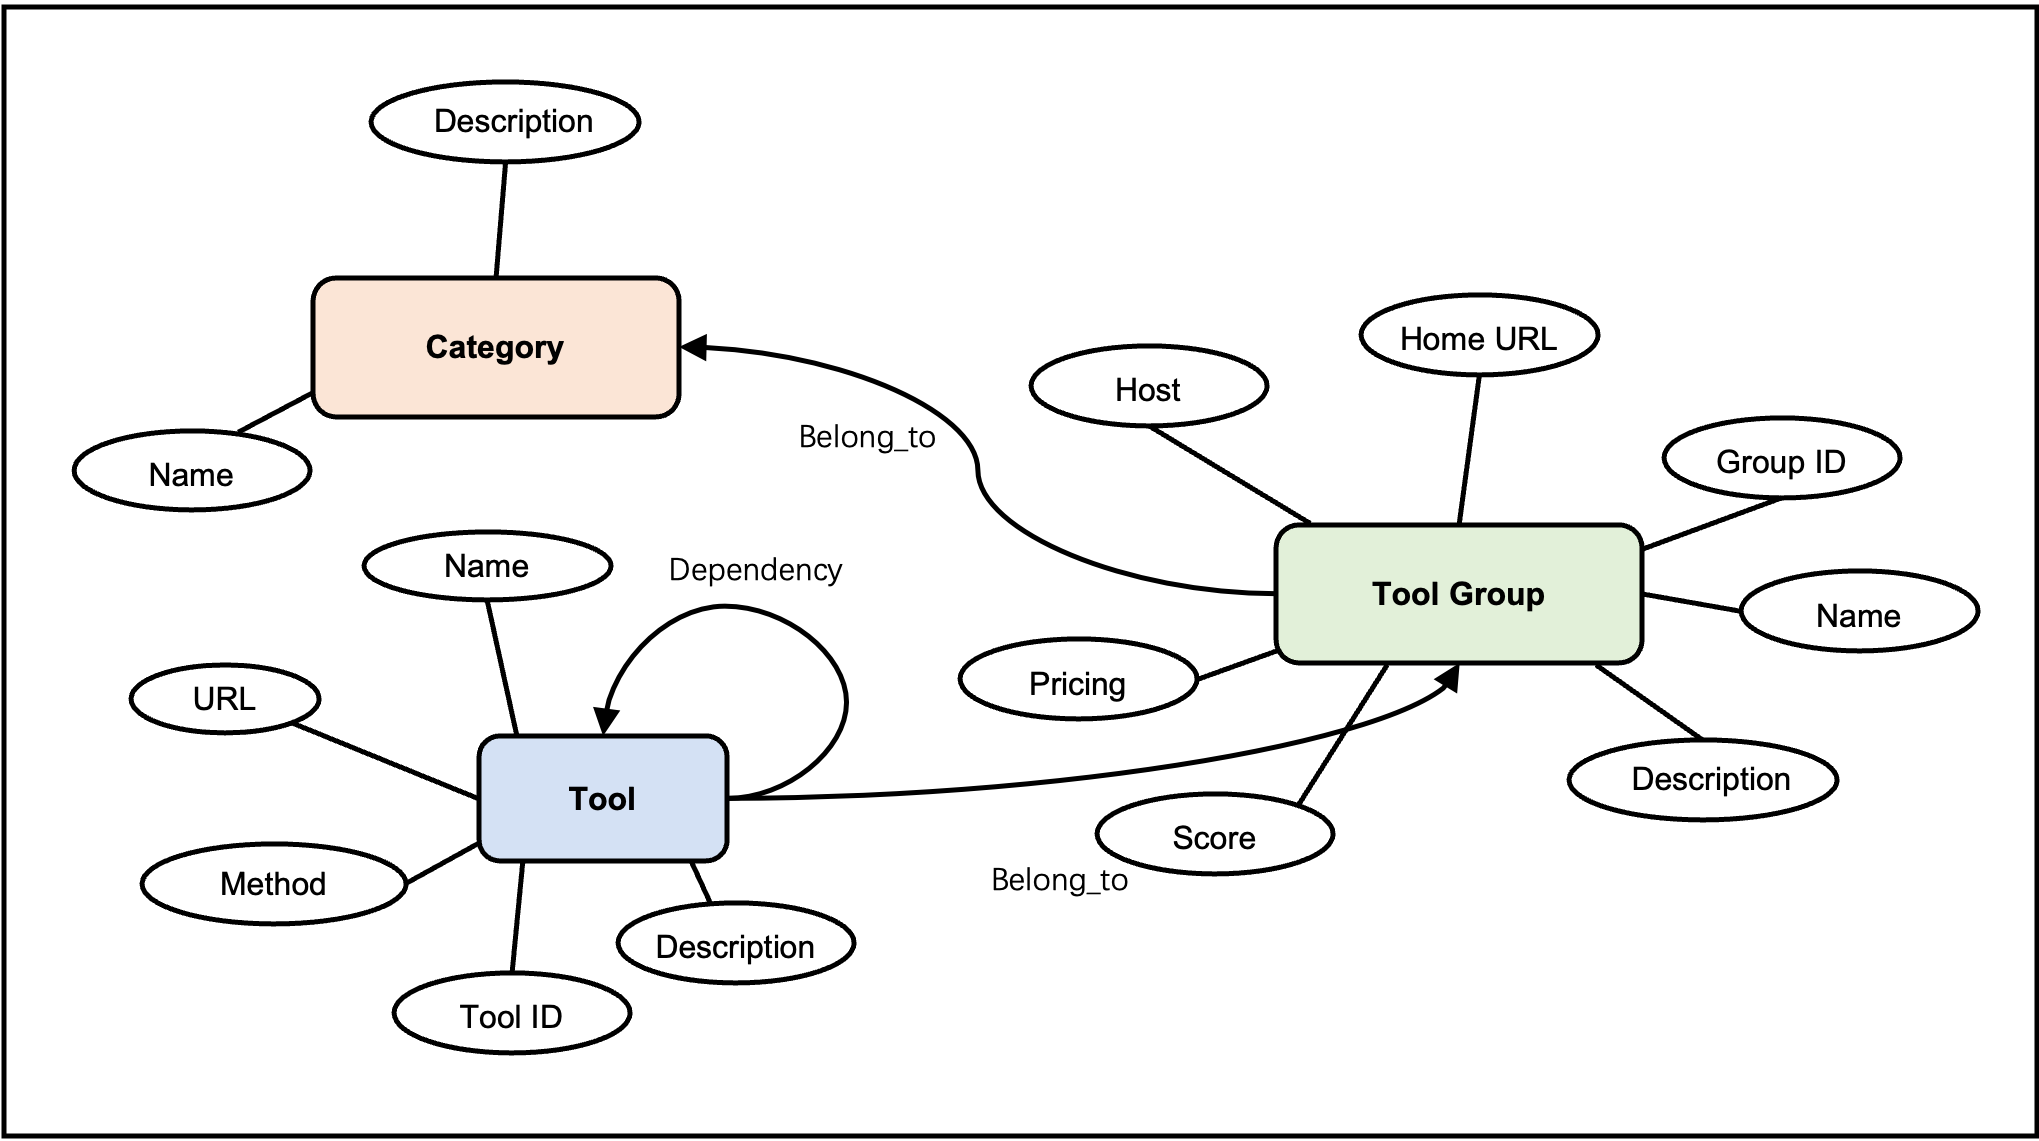
\includegraphics[height=6cm]{../assets/图谱概念模型.png}
    \bicaption{工具图谱概念模型}{Ontology Model of Knowledge Graph}
    \label{fig:ch3-knowledge-graph-ontology-model}
\end{figure}

\subsubsection{工具(Tool)}

工具节点是图谱的基础实体,表示具体的API接口工具。其结构如图\ref{fig:ch3-kg-tool}所示:

\begin{figure}[H]
    \vspace{1em}
    \centering
    \setlength{\abovecaptionskip}{10pt} % 控制图片和caption之间的距离
    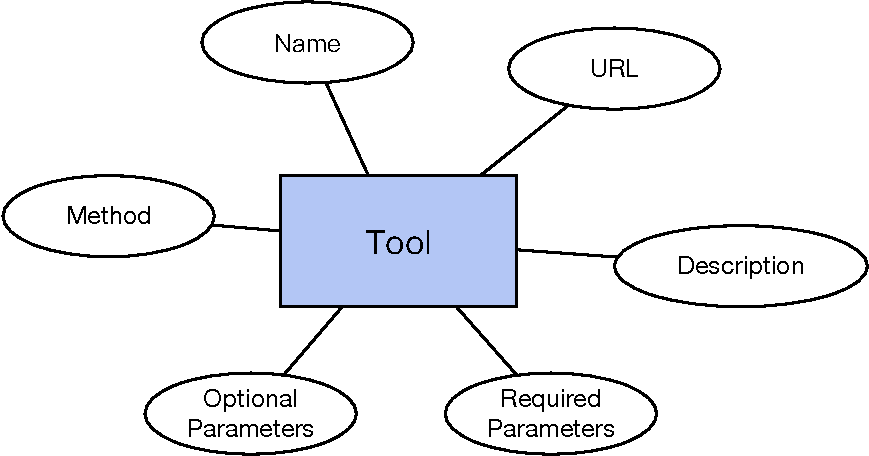
\includegraphics[height=5cm]{../assets/图谱格式-tool.pdf}
    \bicaption{工具实体结构}{Tool Entity Structure}
    \label{fig:ch3-kg-tool}
\end{figure}

\begin{itemize}
    \item Name(名称):工具的唯一标识名称。
    \item URL(接口地址):API工具的访问地址。
    \item Description(描述):工具的简要说明,通常用于描述其用途或功能。
    \item Method(请求方法):支持的HTTP方法,如GET、POST等。
    \item Required Parameters(必需参数):调用API所需的必填参数列表。
    \item Optional Parameters(可选参数):调用API的可选参数列表。
\end{itemize}

在工具图谱的组织中,每个工具节点只属于一个工具组。多个工具可以归属于同一个工具组,从而形成对工具功能的逻辑分类。例如,“酒店搜索”工具和“酒店评论查询”工具都可能属于“旅游服务工具组”。这种一对多的归属关系确保工具图谱结构的清晰性,同时避免工具节点的多重归属问题。

\subsubsection{工具组(Tool Group)}

工具组节点表示一组功能相关的工具的集合,用于组织和分类多个工具节点。其结构如图\ref{fig:ch3-kg-tool-group}所示:

\begin{figure}[H]
    \vspace{1em}
    \centering
    \setlength{\abovecaptionskip}{10pt} % 控制图片和caption之间的距离
    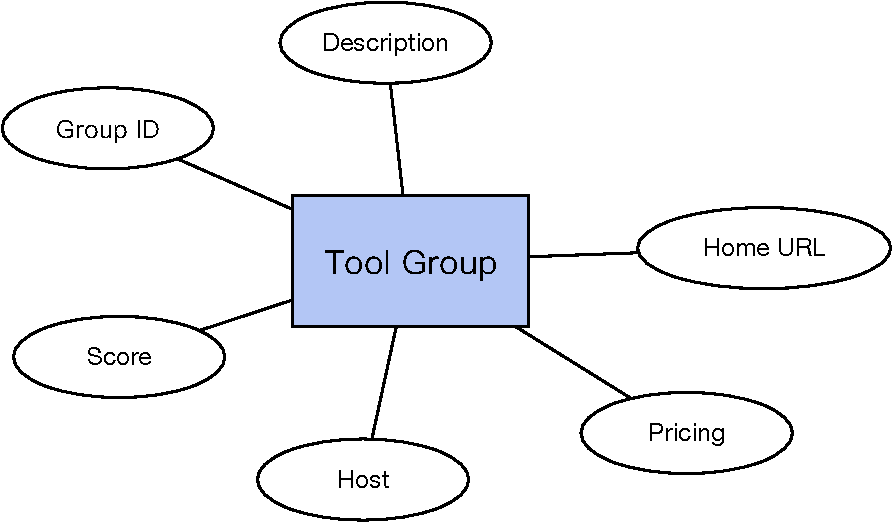
\includegraphics[height=5cm]{../assets/图谱格式-tool group.pdf}
    \bicaption{工具组实体结构}{Tool Group Entity Structure}
    \label{fig:ch3-kg-tool-group}
  \end{figure}

\begin{itemize}
    \item Group ID(工具组ID):工具组的唯一标识符。
    \item Name(名称):工具组的名称。
    \item TDescription(工具组描述):对该工具组的整体描述。
    \item Home URL(链接):工具组的官网链接或信息页面。
    \item Pricing(定价):工具组的定价信息,例如``免费(FREE)''。
    \item Score(评分):工具组的相关指标。
    % ,包括:
    %     \begin{itemize}
    %         \item AvgServiceLevel(服务水平平均值):表示服务稳定性的指标,百分比表示。
    %         \item AvgLatency(平均延迟):工具组调用的平均延迟时间,单位为毫秒。
    %         \item AvgSuccessRate(成功率平均值):表示API调用成功率的平均值,百分比表示。
    %         \item PopularityScore(流行度评分):工具组的受欢迎程度评分。
    %     \end{itemize}
    \item Host(请求地址):工具组所关联的主要域名地址。
\end{itemize}

工具组进一步与工具类别关联,每个工具组只属于一个工具类别,从而实现高层次的分类。例如,“旅游服务工具组”可以归属于“旅游与出行”类别。工具组与工具类别之间的一对多关系,能够有效区分不同工具组的功能领域。

\subsubsection{工具类别(Tool Category)}
工具类别节点表示工具所属的领域、用途或分类。例如,工具类别可以表示工具的主要负责内容为“旅游出行”、“美食”或“电影媒体”。其结构如图\ref{fig:ch3-kg-category}所示:

\begin{figure}[H]
    \vspace{1em}
    \centering
    \setlength{\abovecaptionskip}{10pt} % 控制图片和caption之间的距离
    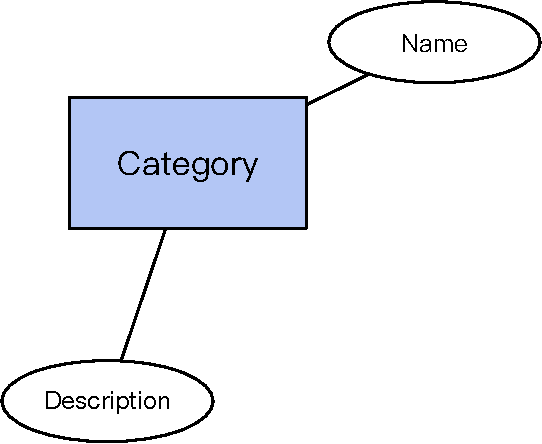
\includegraphics[height=5cm]{../assets/图谱格式-category.pdf}
    \bicaption{工具类别实体结构}{Category Entity Structure}
    \label{fig:ch3-kg-category}
  \end{figure}

\begin{itemize}
    \item Name(名称):类别的名称,用于标识该类别。
    \item Description(描述):对工具类别的简要说明,描述其应用场景或技术范围。
\end{itemize}

工具类别节点与工具组节点的关系是唯一的映射关系,每个工具组只能归属于一个工具类别。此外,工具节点的类别由其所属工具组的类别决定,工具节点和工具组的类别在逻辑上保持一致。这种设计保证了工具图谱的分类层次统一性。例如,“酒店搜索”工具属于“旅游服务工具组”,“旅游服务工具组”属于“旅游与出行”类别,因此“酒店搜索”工具的类别也是“旅游与出行”。

工具之间的依赖关系通常分为三种\cite{shen2023taskbench}:时序依赖、参数依赖、环境依赖。
环境依赖指工具运行所需的外部环境条件(如特定硬件、操作系统或软件版本等)。在本研究中,由于工具多为通过HTTP协议调用的Restful API,不涉及环境依赖。
在参数依赖上,我们进行了一个分类,将参数依赖分为强参数依赖和弱参数依赖两种,下文中将会阐述两者的区别。
因此,本文在工具图谱构建中仅考虑时序依赖和参数依赖两种依赖关系。

在工具图谱的概念模型中,依赖关系主要包括以下三种类型:

\subsubsection{时序依赖(Sequential Dependency)}
时序依赖指的是在历史工具调用路径中被连续调用的两个工具之间的关系。描述如下:
\begin{itemize}
    \item 起点(Source):工具A。
    \item 终点(Target):工具B。
    \item 关系描述(Description):工具B在调用时可能需要工具A的先行调用。
\end{itemize}

\subsubsection{强参数依赖(Strong Resource Dependency)}
强参数依赖指的是某种参数或信息仅能通过前一个工具获取,然后提供给后一个工具。例如,一个旅行商的“酒店ID搜索”工具获取特定的酒店ID,而“酒店评论搜索”工具必须依赖该ID。描述如下:
\begin{itemize}
    \item 起点(Source):工具A。
    \item 终点(Target):工具B。
    \item 参数类型(Resource Type):强依赖的参数类型,例如``酒店ID''。
    \item 关系描述(Description):工具A输出的参数是工具B必须依赖的输入。
\end{itemize}

\subsubsection{弱参数依赖(Weak Resource Dependency)}
弱参数依赖指的是某种参数或信息可以通过另一个工具获取,但不是必须的。例如,“根据经纬度搜索降雨情况”工具可以直接调用,也可以通过“城市经纬度搜索”工具提供经纬度作为输入。描述如下:
\begin{itemize}
    \item 起点(Source):工具A。
    \item 终点(Target):工具B。
    \item 参数类型(Resource Type):弱依赖的参数类型,例如``经纬度''。
    \item 关系描述(Description):工具B的输入可以由工具A提供,但也可以通过其他方式获取。
\end{itemize}

\subsection{基于规则和大语言模型的知识抽取}

本节详细阐述工具知识图谱的构建过程,包括节点和依赖关系的抽取、存储,以及如何将数据导入Neo4j进行存储和查询。

\subsubsection{基于规则的实体抽取}

工具组、工具和工具类别节点的抽取主要依赖规则匹配。从现有的JSON格式工具描述文档中,按照预定义规则通过代码匹配关键信息。工具组的抽取字段包括其ID、工具组名称、工具组描述和主页链接等信息,这些字段为工具组提供全局标识及其关联性。工具节点的提取则更加具体,记录每个工具的名称、API地址、功能描述、HTTP方法(如GET或POST)、必需参数和可选参数等关键信息。工具类别节点用于标识工具组的具体类别,如“天气”、“旅行”等标签,从工具文档中可直接提取。

通过规则提取的节点数据存储为结构化的CSV格式,CSV结构的文件能够直接导入知识图谱,提供了数据的支撑。

\begin{table}[ht]
\centering
\bicaption{工具实体数据格式}{CSV Data Structure for Importing}
\label{tab:csv-example}
\renewcommand{\arraystretch}{1.2}
\scriptsize % 调整字体大小
\begin{tabular}{|l|l|l|p{6cm}|l|}
\hline
\textbf{Category} & \textbf{Product ID} & \textbf{Tool Name} & \textbf{API Description} & \textbf{Hash ID} \\ \hline
Food & \texttt{api\_dcbd91ed...} & Worldwide Recipes & Get detail of recipe & \texttt{167fc042...} \\ \hline
Food & \texttt{api\_dcbd91ed...} & Worldwide Recipes & Get recipes by author & \texttt{d8c4f1e7...} \\ \hline
Food & \texttt{api\_dcbd91ed...} & Worldwide Recipes & Get reviews & \texttt{47f3a387...} \\ \hline
\end{tabular}
\end{table}

\subsubsection{基于规则的时序依赖关系抽取}

时序依赖是通过分析工具调用路径数据来构建的。经过上述的对调用路径的清洗流程,剩下的工具调用数据均可理解为高质量路径。接着,遍历这些调用链中连续调用的工具,将其标记为时序依赖。这种依赖通常用于捕获工具在真实调用路径中的关系,反映调用流程的顺序逻辑。例如,旅行工具链中“酒店搜索”紧接着“酒店评论查询”,这反映了用户实际使用时的时序逻辑,也反映了两者之间的关系。

抽取后的时序依赖关系记录起点工具、终点工具、依赖类型(标记为“时序依赖”)以及描述字段。时序依赖的记录不仅有助于绘制工具调用路径,还为分析流程优化提供依据。

\subsubsection{基于大语言模型的参数依赖关系抽取}

(这是知识图谱有关的关系抽取)
除了通过代码规则抽取工具之间的时序关系,我们还需要对工具之间的参数依赖关系进行分析。
首先,我们尝试了一种基于规则匹配的方案,即通过对工具 API 的输入参数和输出字段进行名称和类别的比对来识别潜在的依赖关系。
这种方法的实现逻辑较为简单直观,对结构化和模式化的依赖关系具有较好的识别能力。
然而,在实际实验中,我们发现该方案存在两个主要问题:

\begin{itemize}
    \item 参数名称不一致导致的依赖关系遗漏。同一参数可能在不同工具中使用不同的名称,例如“酒店ID”在某些工具中可能表示为不同的字段。这种不一致容易导致依赖关系的遗漏,限制了工具知识图谱的表达能力。
    \item 不同语义的同名参数引入的噪声。同名参数在不同工具中可能具有不同的语义。例如,\texttt{ID} 在“酒店搜索”工具中表示“酒店的唯一标识符”,而在“航班搜索”工具中可能指“航班班次编号”。这种情况下,会误判依赖关系,从而引入噪声。
\end{itemize}

尽管规则匹配方法在特定场景下有效,但当面对复杂多样的API数据时,其不足显而易见。此外,人工抽取工具之间的参数依赖关系虽然精确度较高,但成本较高,且难以扩展到大规模工具集成场景。

为解决上述问题,我们引入了大语言模型(LLM)对工具 API 之间的依赖关系进行自动化分析和生成。LLM 凭借其强大的语义理解与解析能力,能够从语义层面识别工具间的参数依赖关系,从而弥补规则匹配的不足。
我们通过将API文档信息融入到LLM的提示词中,并提供相应抽取格式的样本案例,指导大语言模型抽取出API之间的关系和对应参数。

在具体实现中,为了能够完全覆盖工具之间的依赖关系,我们将所有工具两两进行配对,将
工具组名称、工具名称、入参列表、响应体结构等都放在LLM的提示词中,并要求LLM分析
是否存在参数上的依赖关系。若存在参数依赖关系,则输出对应的参数名称并简单描述该依赖关系。

% Set Colors
\definecolor{bgcolor}{RGB}{240,240,240} % Background color
\definecolor{titlecolor}{RGB}{20,20,20} % Title background color

\begin{table}[htbp]
    \centering
    \bicaption{工具图谱关系依赖抽取prompt构建示例}{Example Prompt for Extracting Tool Knowledge Graph's Resource Dependencies} % 表头
    \label{tab:analyze_api_dependencies} % 表格引用标签
    \begin{tcolorbox}[colback=bgcolor, colframe=black, width=0.95\textwidth, boxrule=0.5mm, 
    coltitle=white, colbacktitle=titlecolor, title=Task: Analyze API Dependencies]
    % Centered content
    
    \textbf{<Task>} Analyze the parameter dependencies between two APIs based on their names and descriptions, and output the result in JSON format.
    
    \textbf{<Instructions>}
    1. Identify possible parameter dependencies (e.g., the output of the first tool is the input of the second tool).  
       - If a parameter is unique or organization-specific (e.g., \texttt{product\_id} used internally by Amazon), classify it as a \textbf{strong relationship}.  
       - If a parameter is generic or commonly used (e.g., \texttt{time}, \texttt{longitude}), classify it as a \textbf{weak relationship}.  
    2. Provide a description of the dependency: A concise explanation of what the parameter represents.  
    3. Output the result in JSON format, ensuring it is structured and logically consistent.  
    
    \vspace{0.5em}
    
    \textbf{<API Information>} 

    API1 documentation: \dots

    API2 documentation: \dots 
    
    \vspace{0.5em}
    
    \textbf{<Example Output>}  
    
    \begin{verbatim}
{
    "dependencies": [
    {
        "name_in_first_api": "q",
        "name_in_second_api": "query",
        "dependency_description": "..."
    }
    ]
}
    \end{verbatim}
    
    \end{tcolorbox}
\end{table}

% 引入LLM的方案具能够高效处理参数名称不一致的问题,通过基于上下文语义理解字段的实际含义,避免因名称匹配带来的依赖关系遗漏。同时,LLM还能准确区分参数的语义差异,对于同名字段,可结合工具功能和字段定义的语义信息,明确不同工具中参数的具体含义,从而有效减少噪声。此外,该方案简化了流程并提高了准确性,借助LLM直接生成依赖关系,无需依赖复杂的规则匹配流程,在大规模工具图谱生成中展现出更高的适用性。

图\ref{fig:ch3-knowledge-graph-instance-model}为该工具图谱的实例模型示意图。

\begin{figure}[H]
    \vspace{1em}
    \centering
    \setlength{\abovecaptionskip}{10pt} % 控制图片和caption之间的距离
    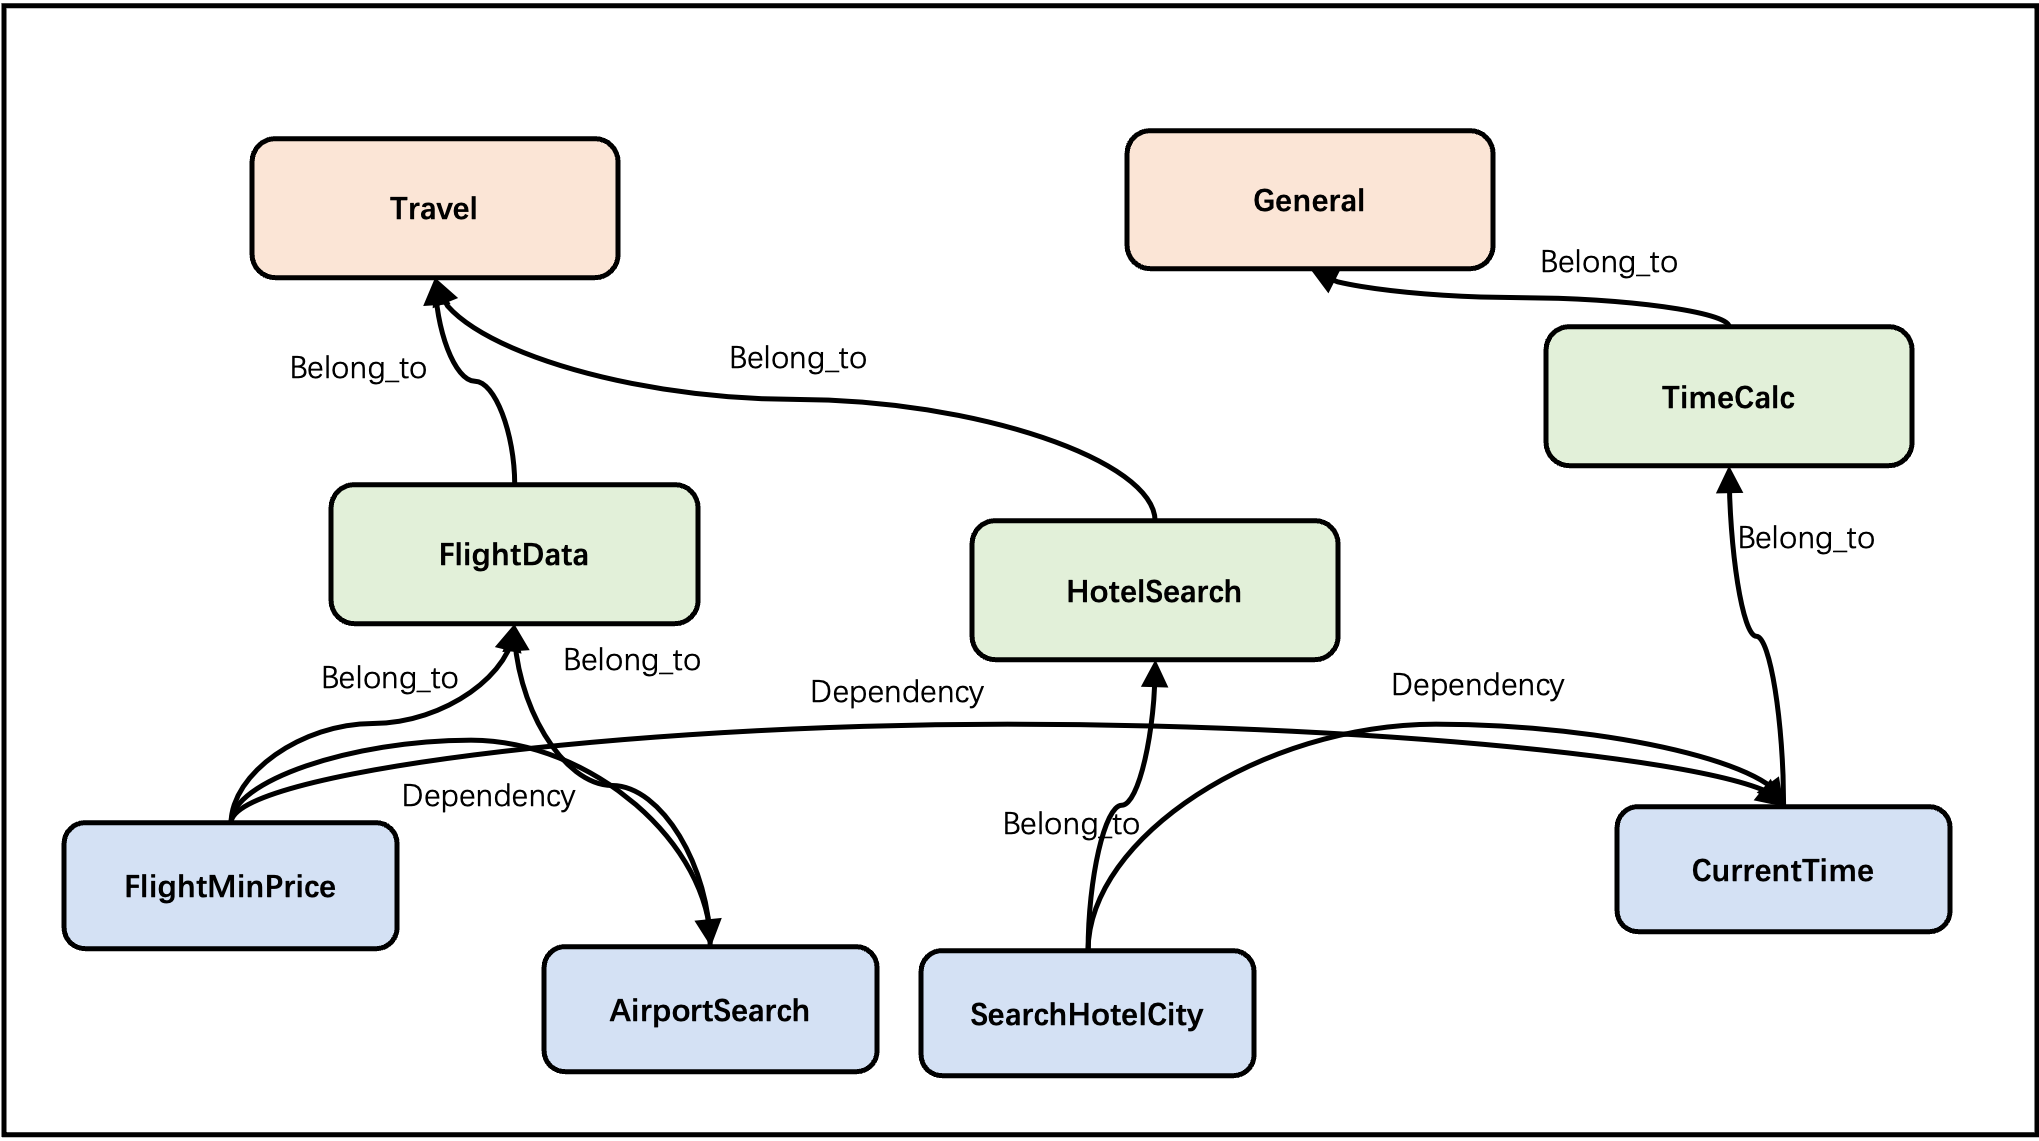
\includegraphics[height=6cm]{../assets/图谱实例模型.png}
    \bicaption{工具图谱实例模型}{Instance Model of Knowledge Graph}
    \label{fig:ch3-knowledge-graph-instance-model}
\end{figure}

总体而言,引入 LLM 的方案,不仅弥补了基于规则匹配的局限性,还通过语义理解能力显著提升了依赖关系识别的全面性和准确性。

\subsection{图谱数据导入}

构建完成的工具知识图谱数据需要导入Neo4j图数据库,以支持高效存储和复杂查询。数据导入分为节点和关系两部分。首先,工具、工具组和工具类别被转化为图中的节点。它们分别通过名称、ID等标识字段建立类型,并与属性字段一一关联。

关系数据的导入使用工具节点的标识字段建立工具之间的依赖关系,包括时序依赖、强参数依赖和弱参数依赖。依赖关系被标注有明确的类型和描述字段,便于在查询中准确反映其性质。
除工具之间的关系,工具与工具组以及工具组与类别之间的关系也被一并导入。
导入完成后,可以通过可视化工具查看图谱中的节点和关系,确保结构的准确性和逻辑性。

导入Neo4j后的结果如图\ref{fig:ch3-neo4j}所示。

\begin{figure}[H]
    \vspace{1em}
    \centering
    \setlength{\abovecaptionskip}{10pt} % 控制图片和caption之间的距离
    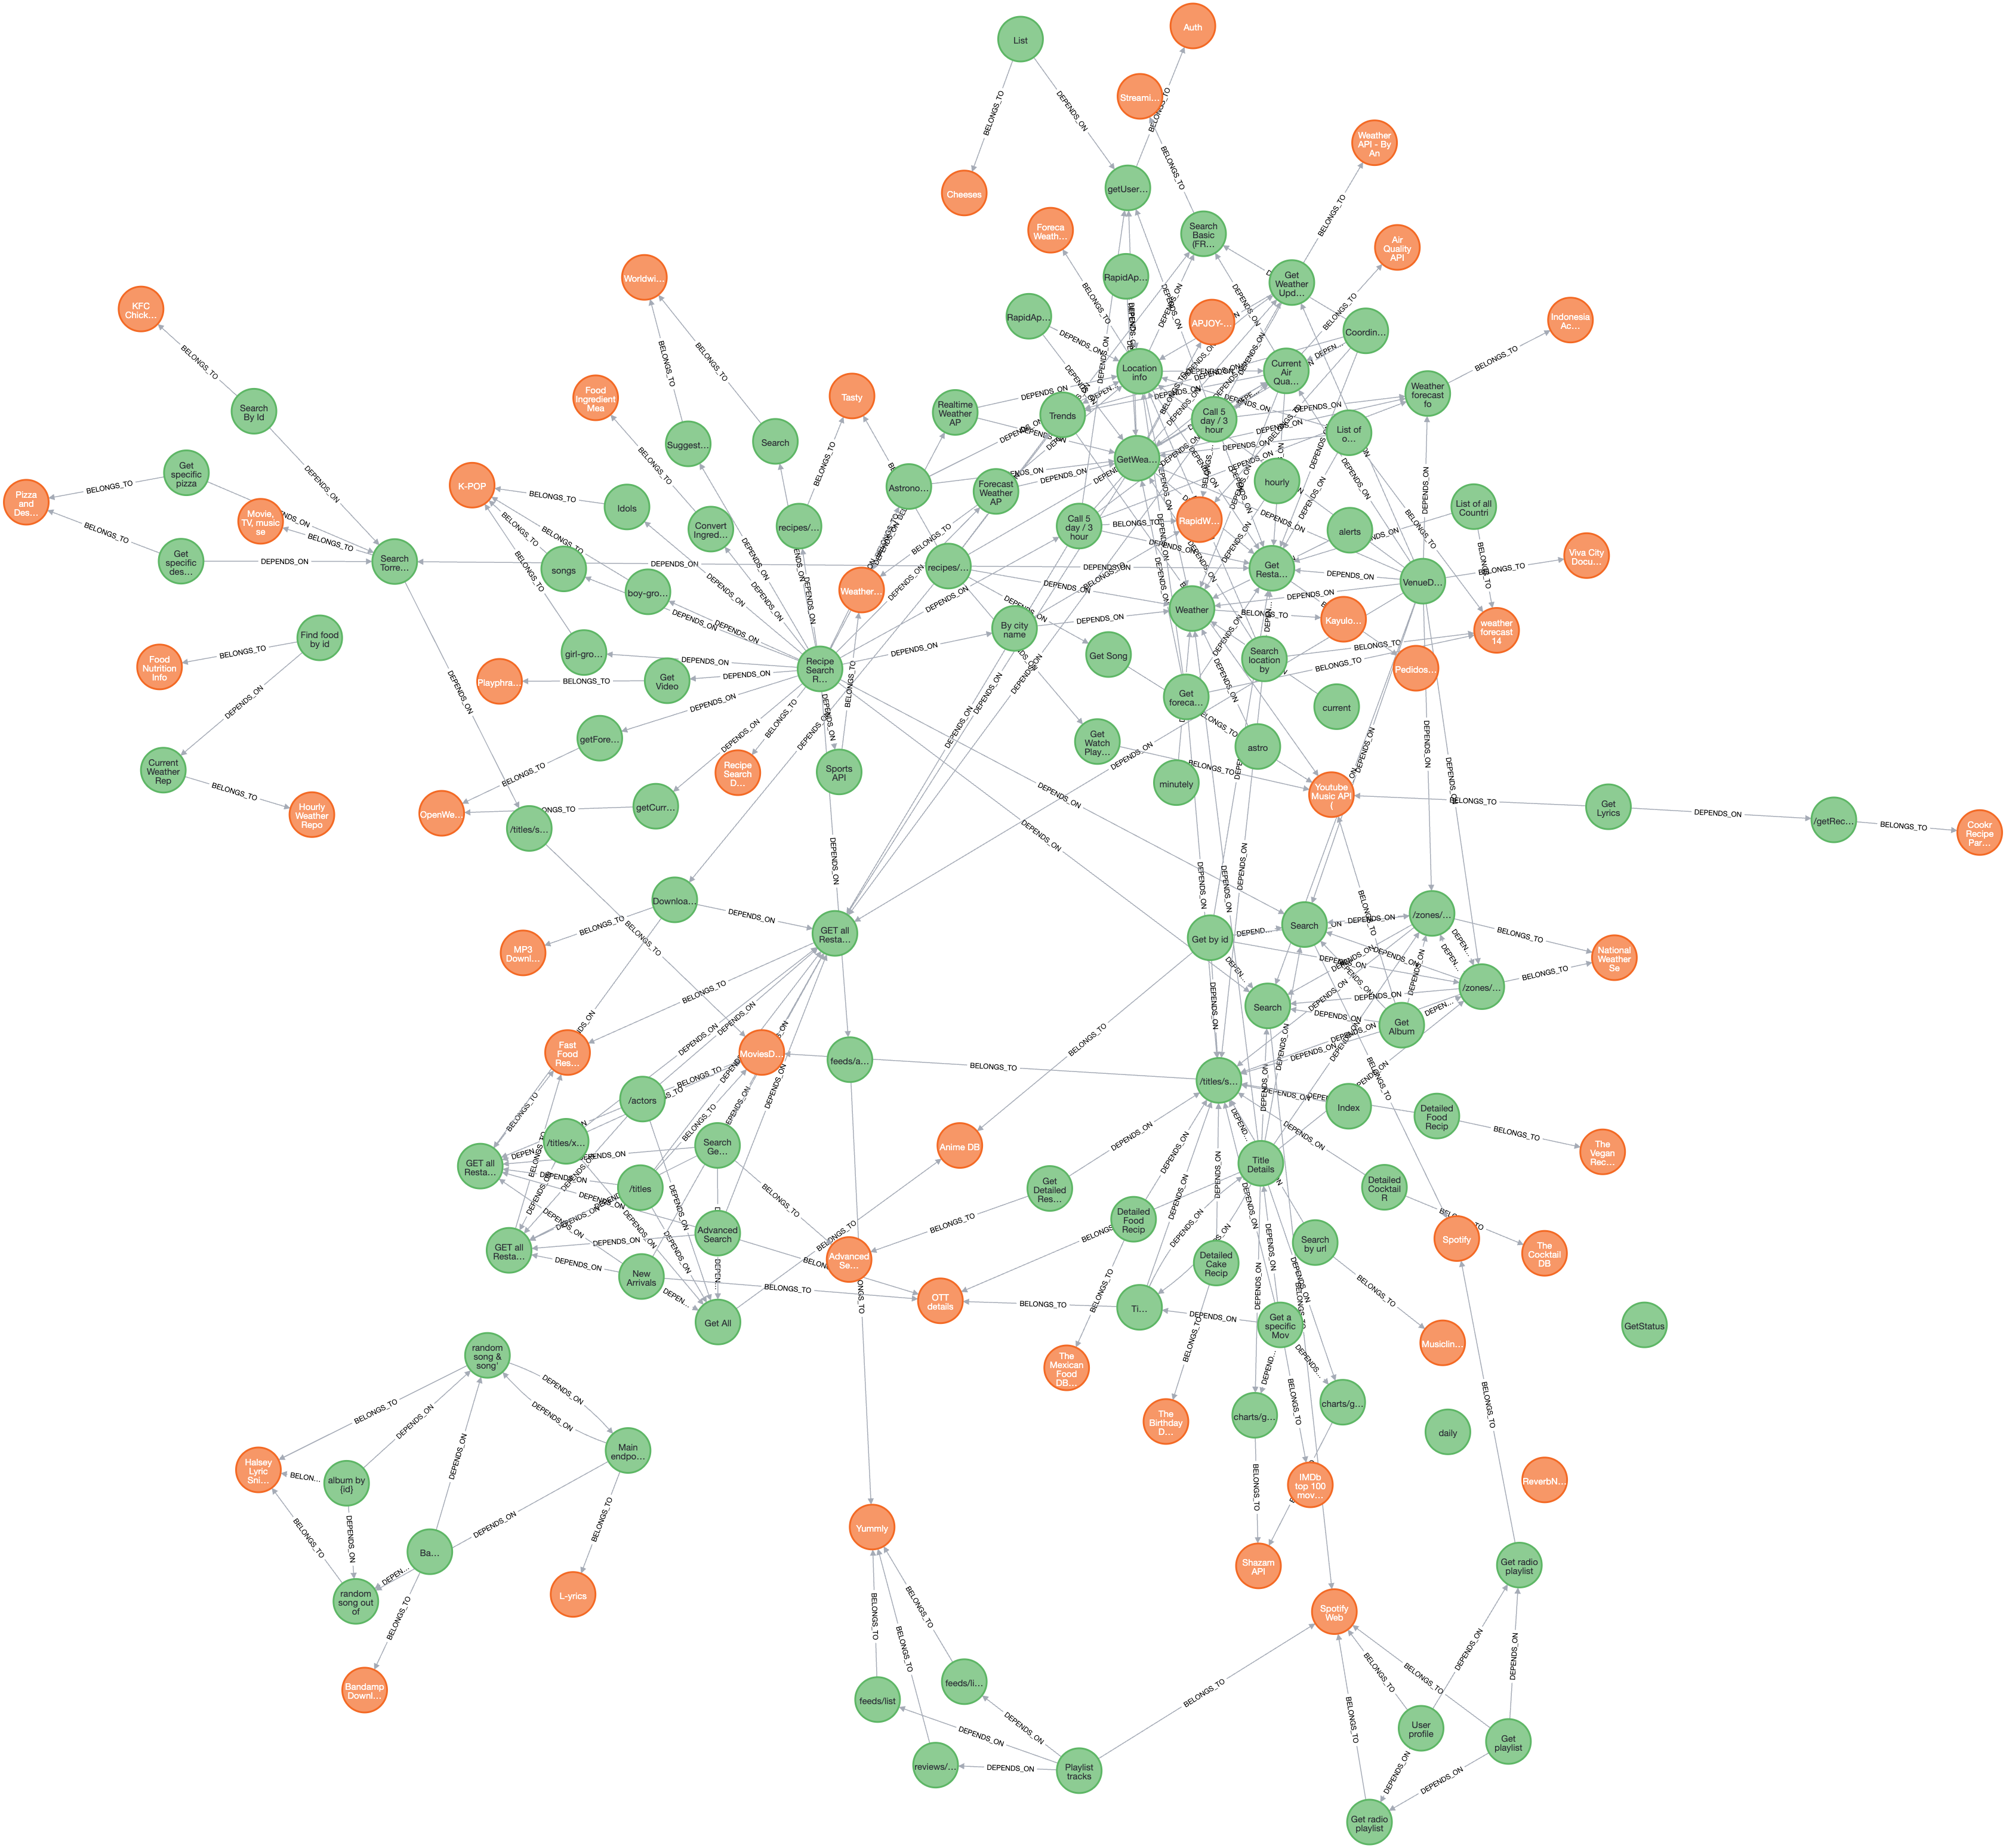
\includegraphics[height=8cm]{../assets/Neo4j工具图1126-150nodes.png}
    \bicaption{工具图谱}{Tool Knowledge Graph}
    \label{fig:ch3-neo4j}
\end{figure}

\subsection{工具图谱更新策略}

工具知识图谱并非建立之后就一成不变,
而是会随着工具的废弃和新增发生变化,
例如工具/工具组的新增和删除。
为了维护图谱的完整性和一致性,
我们设计了一套工具知识图谱更新策略,确保新增工具/工具组能够正确融入现有图谱,同时有效移除无效或过时的工具/工具组。

在删除工具组时,需要从图谱中移除工具组节点及其包含的所有工具节点,
同时删除这些节点与其他节点的所有关联关系。
对于单个工具的删除,则移除对应的工具节点以及该节点与其他工具节点或类别节点之间的关系,
从而避免在图谱中留下无效的孤立边或节点。

\begin{algorithm}[!hpt]

    \bicaption{工具组与工具的删除逻辑伪代码}{Removing Tool Groups and Tools from the Knowledge Graph}
    \label{alg:delete_tool_graph}
    
    \KwIn{工具图谱 \texttt{Graph}, 待删除的工具组或工具标识 \texttt{nodeID}}
    \KwOut{更新后的工具图谱 \texttt{Graph}}

    \BlankLine
    \textbf{Function} \texttt{DeleteToolGroup}(\texttt{Graph}, \texttt{toolGroupID}):\\
    \Indp
        \texttt{tools} $\gets$ \texttt{Graph.getNodesByProperty}("group\_id", \texttt{toolGroupID})\;
        \ForEach{\texttt{tool} $\in$ \texttt{tools}}{
            \texttt{Graph.deleteNodeAndEdges}(\texttt{tool})\;
        }
        \texttt{Graph.deleteNodeAndEdges}(\texttt{toolGroupID})\;
    \Indm
    \BlankLine
    
    \textbf{Function} \texttt{DeleteTool}(\texttt{Graph}, \texttt{toolID}):\\
    \Indp
        \texttt{Graph.deleteNodeAndEdges}(\texttt{toolID})\;
    \Indm
    \BlankLine
    
    \textbf{Main Procedure}:\\
    \Indp
        \If{\texttt{nodeID} \text{ is a tool group ID}}{
            \texttt{DeleteToolGroup}(\texttt{Graph}, \texttt{nodeID})\;
        }
        \ElseIf{\texttt{nodeID} \text{ is a tool ID}}{
            \texttt{DeleteTool}(\texttt{Graph}, \texttt{nodeID})\;
        }
    \Indm
    \end{algorithm}

在添加新工具时,首先将新增工具的相关信息导入图谱。
如果新增工具组尚未存在,则创建对应的工具组节点并将其信息导入,并将其与相关类别节点建立联系。
随后,为每个新增工具节点生成实体,并将工具节点与其所属工具组节点关联,以反映图谱的分类结构。


\begin{algorithm}[!hpt]
\bicaption{工具组与工具的添加逻辑伪代码}{Adding Tool Groups and Tools from the Knowledge Graph}
\label{alg:add_tool_graph}
\KwIn{工具图谱 \texttt{Graph}, 工具组信息 \texttt{toolGroupInfo}, 工具信息列表 \texttt{tools}}
\KwOut{更新后的工具图谱 \texttt{Graph}}

\BlankLine
\textbf{Function} \texttt{AddToolGroup}(\texttt{Graph}, \texttt{toolGroupInfo}, \texttt{tools}):\\
\Indp
    \If{\texttt{!Graph.nodeExists}(\texttt{toolGroupInfo["id"]})}{
        \texttt{Graph.addNode}(\texttt{toolGroupInfo["id"]}, \texttt{toolGroupInfo})\;
        \texttt{Graph.addEdge}(\texttt{toolGroupInfo["id"]}, \texttt{toolGroupInfo["category\_id"]}, \texttt{"belongs\_to"})\;
    }
    \ForEach{\texttt{toolInfo} $\in$ \texttt{tools}}{
        \texttt{AddTool}(\texttt{Graph}, \texttt{toolInfo}, \texttt{toolGroupInfo["id"]})\;
    }
\Indm
\BlankLine

\textbf{Function} \texttt{AddTool}(\texttt{Graph}, \texttt{toolInfo}, \texttt{toolGroupID}):\\
\Indp
    \If{\texttt{!Graph.nodeExists}(\texttt{toolInfo["id"]})}{
        \texttt{Graph.addNode}(\texttt{toolInfo["id"]}, \texttt{toolInfo})\;
        \texttt{Graph.addEdge}(\texttt{toolInfo["id"]}, \texttt{toolGroupID}, \texttt{"belongs\_to"})\;
    }
\Indm
\BlankLine

\textbf{Main Procedure}:\\
\Indp
    \texttt{AddToolGroup}(\texttt{Graph}, \texttt{toolGroupInfo}, \texttt{tools})\;
\Indm
\end{algorithm}

为了完善新增工具的关系,我们对时序依赖关系和参数依赖关系进行分析。
在时序依赖方面,由于新增工具不一定有现成的工具调用路径数据。
因此我们对于新增工具暂不添加时序依赖关系,而是利用新工具
的工具文档等信息来提取参数依赖信息。
在提取强/弱参数依赖的部分,我们采取与上方基于大语言模型的参数依赖关系抽取同样的方式,
将新增工具与现有工具进行两两配对,
分析两个工具之间的参数依赖关系,并根据匹配结果创建工具之间的参数关系。

在自动化更新流程中,删除和添加操作被区分处理。
当进行工具删除时,系统会根据工具或工具组的标识,从图谱中删除相应的节点及其所有关联边。
对于工具添加,系统会自动生成新增工具及工具组的节点信息,并调用参数依赖关系分析模块,更新其与现有图谱中其他工具的关系。

通过上述工具图谱更新策略,工具图谱能够动态适应工具生态的变化,在保证结构一致性的同时,降低了维护的复杂性。这种设计为大规模集成工具的系统提供了稳定可靠的基础支持。


% \begin{itemize}
%   \item 时序依赖:时序依赖指的是在历史工具调用路径中被连续调用的两个工具。
%   \item 强参数依赖:在参数依赖部分,我们根据资源的强弱依赖进行区分。强依赖指的是某种资源/信息仅能通过前一个API工具获取,然后提供给后一个API工具。比如某个旅行商有自己设定的酒店ID,而搜索酒店评论时必须根据该ID来获取,那么在“酒店ID搜索”和“酒店评论搜索”两个工具之间就存在“酒店ID”的强依赖关系。
%   \item 弱参数依赖:弱参数依赖指的是API工具的某种资源/信息可以通过另一个API工具获取,但是不是必须的。比如我们要搜索“根据经纬度搜索降雨情况“时,首先需要获取上海的经纬度。这个经纬度既可以通过大语言模型本身的知识获取,也可以通过”城市经纬度搜索“工具来获取。因此这种参数依赖关系不是必须的,而是可以通过大语言模型、多个API工具提供。
% \end{itemize}

% \subsection{静态构建}

% 静态构建图的过程相对简单,只需要遍历路径数据,并计算每两个节点之间的边权和点权值即可。

% 设定 $D$ 为已完成任务的工具使用路径集合,每条路径由工具使用的顺序构成,

% \[
% \text{Trajectory} = [D_1, D_2, \ldots, D_n]
% \]

% 假设每个工具的调用成功与否是一个二元变量 $x_i$,其中:

% \[
% x_i = 
% \begin{cases} 
% 1, & \text{工具调用成功} \\
% -1, & \text{工具调用失败}
% \end{cases}
% \]

% 为了简化操作,我们将“结束”视为一种普通工具,每个工具都与“结束”工具节点相连,
% 当大语言模型智能体认为要结束调用过程时,就会选择“结束”工具。

% 节点 $v_i$ 到 $v_j$ 的转移权重 $w_{i,j}$ 计算如下:

% \[
% w_{i,j} = \frac{\mathbb{E}_D[1(\text{tool}_s = v_i \land \text{tool}_{s+1} = v_j)]}{\mathbb{E}_D[1(\text{tool}_s = v_i)]}
% \]

% 其中,$\mathbb{E}_D[\cdot]$ 表示对路径集合 $D$ 上的期望操作,$1(\cdot)$ 是指示函数,当条件满足时取值为1,否则为0。
% 该公式计算了工具 $v_i$ 被调用后紧接着调用工具 $v_j$ 的频率。

% 除了关注工具之间的依赖关系,每个单独的工具的可用性和稳定性也是真实场景下重要考虑因素。
% 在工具调用路径中,有一些工具调用会出现无访问权限或访问超时的错误信息。
% 因此我们在工具图中通过对节点的权值进行计算和定义,通过点权来表示该工具的可用性或稳定性。
% 节点 $v_i$ 的可用性权重 $\alpha_i$ 计算如下:

% \[
% \alpha_i = \frac{\sum_{s=1}^{n} 1(x_s = 1 \land \text{tool}_s = v_i)}{\sum_{s=1}^{n} 1(\text{tool}_s = v_i)} \quad (0 \leq \alpha_i \leq 1)
% \]

% 这里,$\alpha_i$ 表示工具 $v_i$ 的调用成功率,是该工具在路径中成功调用的次数与其总调用次数的比值。
% 因此该权值的范围是0-1,越接近1,表示该工具的可用性越高,越接近0,表示该工具的可用性越低。

% \subsubsection{分数映射函数}

% 函数 $f(x)$ 用于将累积分数映射到 $(0, +\infty)$ 的范围内,从而确保在权重更新过程中生成正值。归一化的必要性在于,它能够确保所有工具的表现有效比较,避免负值对权重更新造成不良影响。具体而言,映射函数确保所有工具的权重更新结果均为正值,这对于构建有效的工具图谱至关重要。同时,函数通过灵活处理正负分数,使算法在不同情境下保持良好表现,保持各工具之间的相对表现,从而提升模型的准确性和稳定性。函数定义如下:

% \[
% f(x) :=
% \begin{cases}
% \alpha x + 1, & \text{if } x \geq 0 \\
% e^{\alpha x}, & \text{if } x < 0
% \end{cases}
% \]

% 在这个函数中,$\alpha$ 是控制映射函数行为的超参数。对于正分数,映射为线性函数 $f(x) = \alpha x + 1$,使得得分的正向提升以线性方式反映在权重更新中。对于负分数,映射为指数衰减函数 $f(x) = e^{\alpha x}$,这保证了即使在评分较低的情况下,权重的更新也会保持在一个合理的范围内。

% 通过对筛选后的工具路径数据进行上述计算,我们得到了工具图谱的初始静态图谱。

% \subsection{动态更新}

% 基于上述方法构建的静态工具图谱,本文还提出了对边权和点权的动态更新。
% 动态更新对于工具图谱的构建至关重要,原因主要包括以下几点:
% \begin{itemize}
%   \item \textbf{用户偏好的动态变化}:在实际应用中,随着用户行为的变化,新的调用路径会不断生成。这些新路径反映了用户的真实偏好,因此需要及时添加到工具图谱中,使其能够反映最新的用户需求。
%   \item \textbf{工具的生命周期变化}:工具是动态变化的,随着时间推移,有些工具可能会因为开发者的弃用或其他原因而逐渐失去支持。静态构建无法反映这些变化,而需要通过动态更新来调整图中的边权重,确保图谱能够保持对工具现状的准确表示。
% \end{itemize}

% 动态更新发生的时间节点为系统产生了新的工具调用路径时。

% 以下是对于边权和点权更新的具体阐述,以及对保持分数为正的映射函数的介绍。

% \subsubsection{边权的动态更新}

% 对图 \( G \) 的更新尤为关键。由于可用工具路径的数量有限,我们需要对每一条路径进行细致检查。
% LLM 作为工具的评估者,将整个路径作为输入,评估每个工具节点的表现。

% 我们用 \( \Delta_i^{(n)} \) 表示在第 \( n \) 次迭代中节点 \( v_i \) 的评估得分。
% 节点 \( v_i \) 的累积得分 \( s_i^{(n)} \) 计算如下:

% \[
% s_i^{(n)} = \sum_{k=1}^{n} \Delta_i^{(k)}
% \]

% 该公式对节点 \( v_i \) 在每次迭代中的评分进行累积,为后续的转移权重更新提供基础。

% 节点 \( v_i \) 到 \( v_j \) 的转移权重 \( w_{i,j}^{(n)} \) 在第 \( n \) 次迭代中的更新公式如下:

% \[
% w_{i,j}^{(n)} = \beta w_{i,j}^{(0)} + (1 - \beta) \Delta w_{i,j}^{(n)}
% \]

% 其中,\( w_{i,j}^{(0)} \) 是初始的转移权重,\( \beta \) 是控制初始权重与动态更新之间平衡的超参数,\( \Delta w_{i,j}^{(n)} \) 是用于更新转移权重的归一化梯度,计算公式如下:

% \[
% \Delta w_{i,j}^{(n)} = \frac{f(s_i^{(n)})}{\sum_{v_j \in \text{oneigh}(v_i)} f(s_j^{(n)})}
% \]

% 该公式通过累积分数 \( s_i^{(n)} \) 和 \( s_j^{(n)} \) 来更新转移权重,确保工具之间的转移反映最新的评估结果。

% \subsubsection{点权的动态更新}

% 在点权的动态更新中,我们通过分析新生成的工具调用路径来调整工具的可用性权重。设调用路径为:

% \[
% \text{Trajectory} = [D_1, D_2, \ldots, D_n]
% \]

% 对于每个工具 \( D_i \) 的调用结果记作 \( x_i \),其中:

% - \( x_i = -1 \) 表示调用出错,
% - \( x_i = +1 \) 表示调用成功。

% 在这里,出错的调用情况指的是 API 工具本身存在可用性问题,例如遇到状态码“403 Forbidden”、“408 Request Timeout”等。

% 根据调用结果,我们可以对点权的分数进行更新。更新公式如下:

% \[
% v_i^{(n)} = \beta v_i^{(0)} + (1 - \beta) \Delta v_i^{(n)}
% \]

% 其中:
% - \( v_i^{(0)} \) 是工具 \( D_i \) 的初始权重,
% - \( \beta \) 是控制初始权重与动态更新之间平衡的超参数,其值会根据错误信息的严重程度进行调整,
% - \( \Delta v_i^{(n)} \) 是用于更新权重的归一化梯度,计算公式如下:

% \[
% \Delta v_i^{(n)} = \frac{f(s_i^{(n)})}{\sum_{D_j \in \text{oneigh}(D_i)} f(s_j^{(n)})}
% \]

% 在此公式中,$f(s_i^{(n)})$ 是累积分数,通过反映工具 \( D_i \) 的评估结果,确保工具之间的转移权重反映最新的使用情况和反馈。

% \subsection{图谱数据导入}

% 通过上述操作,我们已经得到了构建工具图谱的原始数据,接下来我们需要将改数据转为供Neo4j存储的图谱数据。具体实现如下所示:



% \section{插图}

% 插图功能是利用 \TeX{} 的特定编译程序提供的机制实现的,不同的编译程序支持不同的图
% 形方式。有的同学可能听说“\LaTeX{} 只支持 EPS”,事实上这种说法是不准确的。\XeTeX{}
% 可以很方便地插入 EPS、PDF、PNG、JPEG 格式的图片。

% 一般图形都是处在浮动环境中。之所以称为浮动是指最终排版效果图形的位置不一定与源文
% 件中的位置对应,这也是刚使用 \LaTeX{} 同学可能遇到的问题。如果要强制固定浮动图形
% 的位置,请使用 \pkg{float} 宏包,它提供了 \texttt{[H]} 参数。

% \subsection{单个图形}

% 图要有图题,研究生图题采用中英文对照,并置于图的编号之后,图的编号和图题应置于图
% 下方的居中位置。引用图应在图题右上角标出文献来源。文中必须有关于本插图的提示,如
% “见图~\ref{fig:energy-distrib}”、“如图~\ref{fig:energy-distrib} 所示”等。该页空
% 白不够排写该图整体时,则可将其后文字部分提前排写,将图移到次页。

% \begin{figure}[H]
%   \centering
%   \begin{tikzpicture}
%     \begin{axis}[
%       width=12cm,
%       height=9cm,
%       xmin=0, xmax=7,
%       xlabel={$r$ (\unit{\milli\metre})},
%       ymin=-1000, ymax=11000,
%       ylabel={Energy (\unit[per-mode=symbol]{\watt\per\cubic\metre})},
%       scaled ticks=false,
%       tick label style={
%         /pgf/number format/1000 sep=,
%         font={\zihao{-5}},
%       },
%       minor tick num=1,
%       tick pos=left,
%       tick align=outside,
%       tick style={thin,black},
%     ]
%       \addplot [only marks,mark=square*] 
%         table [x={radial}, y={energy}, col sep=comma] 
%         {./assets/energy-distrib.csv};
%       \node at (2,6000) 
%         {$q_{v}=\dfrac{\sigma\omega^{2}|\mathbf{A}|^{2}}{2}$};
%     \end{axis}
%   \end{tikzpicture}
%   \bicaption{内热源沿径向的分布}{Energy distribution along radial}
%   \label{fig:energy-distrib}
% \end{figure}

% \subsection{多个图形}

% 简单插入多个图形的例子如图~\ref{fig:SRR} 所示。这两个水平并列放置的子图共用一个
% 图形计数器,没有各自的子图题。

% \begin{figure}[H]
%   \centering
%   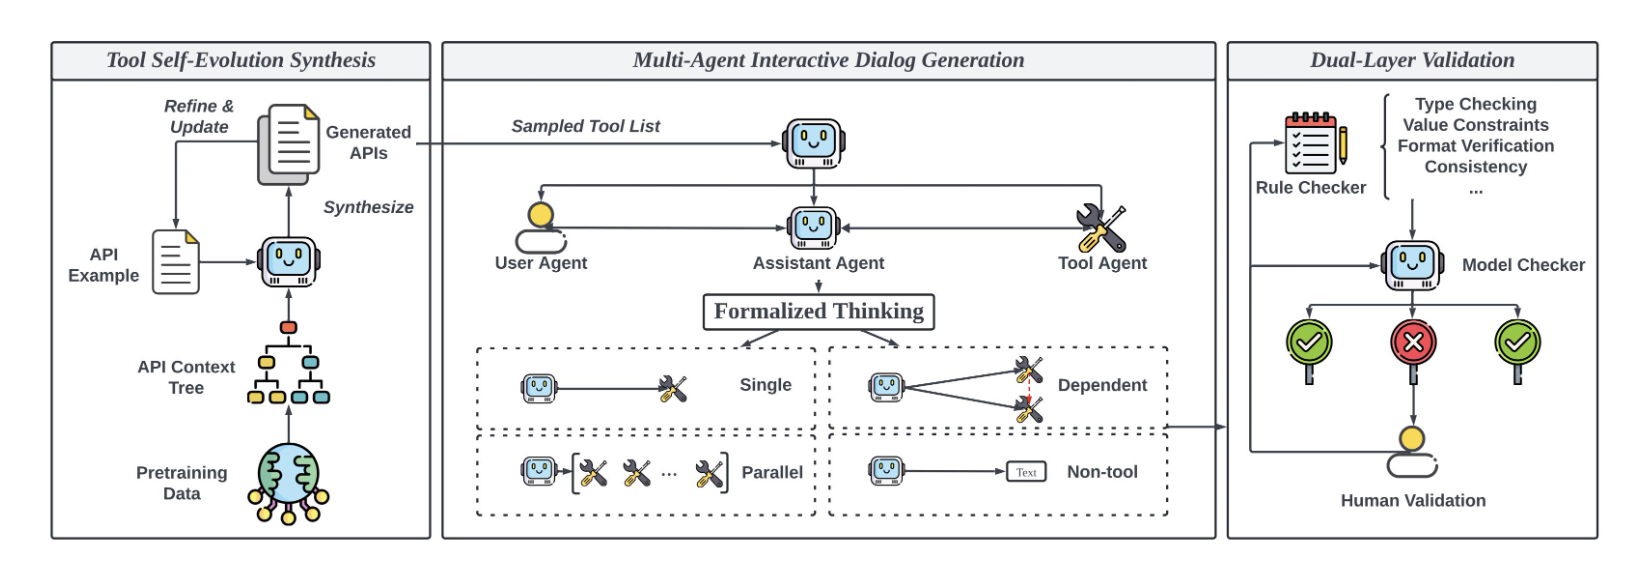
\includegraphics[height=2cm]{../assets/1.png}
%   \hspace{1cm}
%   \includegraphics[height=2cm]{sjtu-vi-badge-red.pdf}
%   \bicaption{中文题图}{English caption}
%   \label{fig:SRR}
% \end{figure}

% 如果多个图形相互独立,并不共用一个图形计数器,那么用 \texttt{minipage} 或者
% \texttt{parbox} 就可以,如图~\ref{fig:parallel1} 与图~\ref{fig:parallel2}。

% \begin{figure}[H]
%   \centering
%   \begin{minipage}{0.48\textwidth}
%     \centering
%     \includegraphics[height=1.7cm]{sjtu-vi-name-red.pdf}
%     \caption{并排第一个图}
%     \label{fig:parallel1}
%   \end{minipage}\hfill
%   \begin{minipage}{0.48\textwidth}
%     \centering
%     \includegraphics[height=1.7cm]{sjtu-vi-name-red.pdf}
%     \caption{并排第二个图}
%     \label{fig:parallel2}
%   \end{minipage}
% \end{figure}

% 如果要为共用一个计数器的多个子图添加子图题,建议使用较新的 \pkg{subcaption} 宏
% 包,不建议使用 \pkg{subfigure} 或 \pkg{subfig} 等宏包。

% 推荐使用 \pkg{subcaption} 宏包的 \cs{subcaptionbox} 并排子图,子图题置于子图之
% 下,子图号用 a)、b) 等表示。也可以使用 \pkg{subcaption} 宏包的 \cs{subcaption}
% (放在 minipage中,用法同 \cs{caption})。

% \pkg{subcaption} 宏包也提供了 \pkg{subfigure} 和 \pkg{subtable} 环境,如
% 图~\ref{fig:subfigure}。

% \begin{figure}[H]
%   \centering
%   \begin{subfigure}{0.3\textwidth}
%     \centering
%     \includegraphics[height=2cm]{sjtu-vi-badge-red.pdf}
%     \caption{校徽}
%   \end{subfigure}
%   \hspace{1cm}
%   \begin{subfigure}{0.4\textwidth}
%     \centering
%     \includegraphics[height=1.7cm]{sjtu-vi-name-red.pdf}
%     \caption{校名。注意这个图略矮些,subfigure 中同一行的子图在顶端对齐。}
%   \end{subfigure}
%   \caption{包含子图题的范例(使用 subfigure)}
%   \label{fig:subfigure}
% \end{figure}

% 搭配 \pkg{bicaption} 宏包时,可以启用 \cs{subcaptionbox} 和 \cs{subcaption} 的双
% 语变种 \cs{bisubcaptionbox} 和 \cs{bisubcaption},如图~\ref{fig:bisubcaptionbox}
% 所示。

% \begin{figure}[!hbtp]
%   \centering
%   \bisubcaptionbox{$R_3 = 1.5\text{mm}$ 时轴承的压力分布云图}%
%                   {Pressure contour of bearing when $R_3 = 1.5\text{mm}$}%
%                   [6.4cm]{\includegraphics[height=3cm]{example-image-a.pdf}}
%   \hspace{1cm}
%   \bisubcaptionbox{$R_3 = 2.5\text{mm}$ 时轴承的压力分布云图}%
%                   {Pressure contour of bearing when $R_3 = 2.5\text{mm}$}%
%                   [6.4cm]{\includegraphics[height=3cm]{example-image-b.pdf}}
%   \bicaption{包含子图题的范例(使用 subcaptionbox)}
%             {Example with subcaptionbox}
%   \label{fig:bisubcaptionbox}
% \end{figure}


% \section{表格}

% \subsection{基本表格}

% 编排表格应简单明了,表达一致,明晰易懂,表文呼应、内容一致。表题置于表上,研究生
% 学位论文可以用中、英文两种文字居中排写,中文在上,也可以只用中文。

% 表格的编排建议采用国际通行的三线表\footnote{三线表,以其形式简洁、功能分明、阅读
% 方便而在科技论文中被推荐使用。三线表通常只有 3 条线,即顶线、底线和栏目线,没有
% 竖线。}。三线表可以使用 \pkg{booktabs} 提供的 \cs{toprule}、\cs{midrule} 和
% \cs{bottomrule}。它们与 \pkg{longtable} 能很好的配合使用。


% \begin{table}[!hpt]
%   \caption[一个颇为标准的三线表]{一个颇为标准的三线表\footnotemark}
%   \label{tab:firstone}
%   \centering
%   \begin{tabular}{@{}llr@{}} \toprule
%     \multicolumn{2}{c}{Item} \\ \cmidrule(r){1-2}
%     Animal & Description & Price (\$)\\ \midrule
%     Gnat  & per gram  & 13.65 \\
%           & each      & 0.01 \\
%     Gnu   & stuffed   & 92.50 \\
%     Emu   & stuffed   & 33.33 \\
%     Armadillo & frozen & 8.99 \\ \bottomrule
%   \end{tabular}
% \end{table}
% \footnotetext{这个例子来自
%   \href{https://mirrors.sjtug.sjtu.edu.cn/ctan/macros/latex/contrib/booktabs/booktabs.pdf}%
%   {《Publication quality tables in LaTeX》}(\pkg{booktabs} 宏包的文档)。这也是
%   一个在表格中使用脚注的例子,请留意与 \pkg{threeparttable} 实现的效果有何不
%   同。}

% \subsection{复杂表格}

% 我们经常会在表格下方标注数据来源,或者对表格里面的条目进行解释。可以用
% \pkg{threeparttable} 实现带有脚注的表格,如表~\ref{tab:footnote}。

% \begin{table}[Hb]
%   \bicaption{一个带有脚注的表格的例子}{A Table with footnotes}
%   \label{tab:footnote}
%   \centering
%   \begin{threeparttable}[b]
%      \begin{tabular}{ccd{4}cccc}
%       \toprule
%       \multirow{2}*{total} & \multicolumn{2}{c}{20\tnote{a}} & \multicolumn{2}{c}{40} & \multicolumn{2}{c}{60} \\
%       \cmidrule(lr){2-3}\cmidrule(lr){4-5}\cmidrule(lr){6-7}
%       & www & \multicolumn{1}{c}{k} & www & k & www & k \\ % 使用说明符 d 的列会自动进入数学模式,使用 \multicolumn 对文字表头做特殊处理
%       \midrule
%       & $\underset{(2.12)}{4.22}$ & 120.0140\tnote{b} & 333.15 & 0.0411 & 444.99 & 0.1387 \\
%       & 168.6123 & 10.86 & 255.37 & 0.0353 & 376.14 & 0.1058 \\
%       & 6.761    & 0.007 & 235.37 & 0.0267 & 348.66 & 0.1010 \\
%       \bottomrule
%     \end{tabular}
%     \begin{tablenotes}
%     \item [a] the first note.
%     \item [b] the second note.
%     \end{tablenotes}
%   \end{threeparttable}
% \end{table}


% \section{算法环境}

% 算法环境可以使用 \pkg{algorithms} 宏包或者较新的 \pkg{algorithm2e} 实现。
% 算法~\ref{algo:algorithm} 是一个使用 \pkg{algorithm2e} 的例子。关于排版算法环境
% 的具体方法,请阅读相关宏包的官方文档。

% \begin{algorithm}[htb]
%   \caption{算法示例}
%   \label{algo:algorithm}
%   \small
%   \SetAlgoLined
%   \KwData{this text}
%   \KwResult{how to write algorithm with \LaTeXe }

%   initialization\;
%   \While{not at end of this document}{
%     read current\;
%     \eIf{understand}{
%       go to next section\;
%       current section becomes this one\;
%     }{
%       go back to the beginning of current section\;
%     }
%   }
% \end{algorithm}


\section{本章小结}

本章提出了一种结合规则方法和大语言模型的工具图谱构建方法,系统化地完成了从工具数据筛选到概念模型设计再到数据导入的全流程。首先,为构建高质量的图谱数据基础,我们设计了两种数据筛选策略,对工具描述信息和调用路径数据进行筛选,提取出高质量的工具集合和调用路径。在图谱结构设计方面,定义了工具图谱的核心概念模型,包含工具节点、工具组节点和工具类别节点,并明确了它们之间的层次关系和依赖结构。通过建模时序依赖、强参数依赖和弱参数依赖三种关系,详细描述了工具之间的调用逻辑。根据上述方法,本文成功构建出高质量的工具图谱,并将其导入Neo4j数据库,实现了图谱的可视化和高效查询,为复杂任务场景下的工具调用和规划提供了强有力的支持。
为了适应开源工具的实时性和持续变化的工具生态,本章还提出了对工具图谱进行更新的方法,并针对删除和添加工具两种情况进行了介绍。
